\usetikzlibrary{mindmap,trees}
\titleSlide
\inuitsSlide

\frame{%
    \frametitle{whoami}
    \framesubtitle{Julien Pivotto}
    \begin{itemize}
        \item{System administrator at {\inuits{}inuits\small.eu}}
        \item{Git user for 5+ years}
        \item{DevOps believer}
        \item{Open-source defender since 2004}
        \olditem{\textit{\ctr{@roidelapluie}} \ctr{on irc/twitter/github}}
    \end{itemize}
}


\frame{%
    \frametitle{Ops <3 Dev}
    \begin{itemize}
        \item{Infrastructure as Code}
            \begin{itemize}
                \item SCM all the things
                \item Monitoring
                \item Configuration
                \item Application deployment
                \end{itemize}
        \item{Taking part of software development}
            \begin{itemize}
                \item Understanding
                \item Monitoring
                \item High Availability
                \item \dots
            \end{itemize}
    \end{itemize}
}

\frame{%
    \frametitle{Me and git}
    \begin{itemize}
        \item{I first used subversion (10 years ago)}
        \item{Private forges and sourceforge}
        \item{5 years later a lot of projects moved to git}
        \item{The Puppet community also uses a lot git}
        \item Git/Hg are the de-facto standards in OS projects
    \end{itemize}
}


\begin{frame}
    \begin{center}
        
\includegraphics[height=2cm]{git.png}
    \end{center}
    \begin{center}
        Git is a free and open source\pause{} distributed\pause{} version control system\pause{} designed to handle everything from small to very large projects\pause{} with speed and efficiency.
    \end{center}
    \begin{flushright}
        Source: http://git-scm.com/
    \end{flushright}
\end{frame}
\begin{frame}
    \frametitle{git log}
    \begin{itemize}
        \item{Initiated in 2005 by Linus Torvalds}
        \item{Replacement of closed-source BitKeeper}
        \item{Created for the Linux Kernel development}
        \item{Now used by thousands of projects}
    \end{itemize}
\end{frame}
\begin{frame}
    \frametitle{git is distributed}
    \begin{itemize}
        \item Everything can be done in local (except pull\&push)
        \item Work with several remotes
        \item Share code with anyone
        \item No unique central repository
        \item A lot of workflows possible
    \end{itemize}
\end{frame}
\begin{frame}
    \frametitle{Branching and merging is easy}
    \begin{itemize}
        \item You can branch locally
        \item Merging is easy and simple
        \item You can squash commits
    \end{itemize}
\end{frame}
\begin{frame}
    \frametitle{How to access a repo}
    \begin{itemize}
        \item Locally (Local filesystems)
        \item SSH
        \item HTTP/HTTPs
        \item Git protocol
    \end{itemize}
\end{frame}
\begin{frame}
    \frametitle{git is open-source}
    \begin{itemize}
        \item Published under GPL-2\pause
        \item Written in C\pause
        \item A lot of frontends/backends
        \item A lot of libraries
        \item A lot of hosting services
        \item And a lot of users
    \end{itemize}
\end{frame}


\begin{iframe}[A team]
\item One person
\item 100 people
\item Coders, testers, readers?
\end{iframe}

\begin{iframe}[Git is your code]
\item Full of information
\item Code changes
\item Commit messages
\item Dates
\item Branches
\item Tags
\end{iframe}


\CenterSlide{The Commit Message}


\begin{iframe}[The commit message]
\item One short first line
\item Longer description
\item Ticket number
\end{iframe}


\frame{%
    \begin{center}
    \tikzset{every node/.append style={scale=0.7,font=\os}}
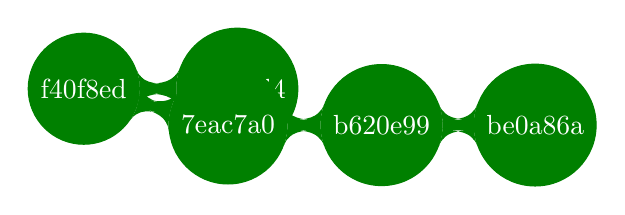
\begin{tikzpicture}
    \path[concept color=green!50!black,text=white, yscale=0.9,xscale=1.3]
    node[concept, color=green!50!black,text=white,level distance=1cm] {f40f8ed}
    [clockwise from=0]
    child[concept color=green!50!black] {node[concept]{66c2ad4}}
    child[concept color=green!50!black] {
        %[clockwise from=45]
        node[concept]{7eac7a0}
    }
    [clockwise from=0]
    child[concept color=green!50!black] {node[concept]{b620e99}}
    [clockwise from=0]
    child[concept color=green!50!black] {node[concept]{be0a86a}};
    \end{tikzpicture}
\end{center}
}

%f40f8ed
%0db443e
%b620e99
%be0a86a
%183bca9
%7eac7a0
%d0b3417
%66c2ad4
%ffc575c
%c692cc3

% quickintro
% basics
% commit message vs project management
% git blame
% git stash
% workflows
% git squash
% git merge

\thankyouSlide
\renewcommand{\insertLogo}{}
\contactSlide
